

\chapter{Retas e Planos}\label{cap_estudo}
\badgeRevisar

A geometria analítica é uma área interdisciplinar da matemática que faz o estudo de objetos da geometria através de estruturas algébricas (equações e inequações algébricas). Para tanto, o primeiro passo é a construção (definição) de um sistema de coordenadas, no qual os objetos geométricos serão referenciados.

Dado um sistema de coordenadas podemos fazer o equacionamento de elementos geométricos como retas e planos.

\section{Sistema de coordenadas no espaço}\label{cap_estudo_sec_scoord}
\badgeRevisar

\badgeYouTube{aZZ1OmEj4T0}
% \begin{flushright}
%   \href{https://archive.org/details/sistema-de-coordenadas-tridimensional}{$\blacktriangleright$ Vídeo disponível!}
% \end{flushright}

Um sistema de coordenadas (cartesianas\descartes) no espaço é constituído de um ponto $O$ e uma base de vetores $B = (\vec{e}_1, \vec{e}_2, \vec{e}_3)$ no espaço. Dado um tal sistema, temos que cada ponto $P$ determina de forma única um vetor $\overrightarrow{OP} = (x,y,z)$ e vice-versa. Assim sendo, definimos que o ponto $P$ tem coordenadas $(x,y,z)$. Veja a figura abaixo.

\begin{figure}[H]
  \centering
  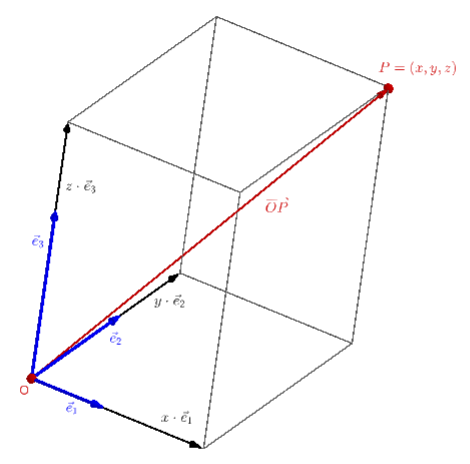
\includegraphics[width=0.8\textwidth]{cap_estudo/dados/fig_scoord/fig}
  \caption{Ilustração de um sistema de coordenadas no espaço.}
  \label{fig:scoord}
\end{figure}

O ponto $O$ é chamado de \emph{origem} (do sistema de coordenadas) e tem coordenadas $O=(0,0,0)$. Dado um ponto $P=(x,y,z)$, chama-se $x$ de sua \emph{abscissa}, $y$ de sua \emph{ordenada} e $z$ de sua \emph{cota}. As retas que passam por $O$ e têm, respectivamente, as mesmas direções de $\vec{e}_1$, $\vec{e}_2$ e $\vec{e}_3$ são chamadas de \emph{eixo das abscissas}, \emph{eixo das ordenadas} e \emph{eixo das cotas}. Os planos que contém $O$ e representantes de dois vetores da base $B$ são chamados de \emph{planos coordenados}.

\begin{figure}[H]
  \centering
  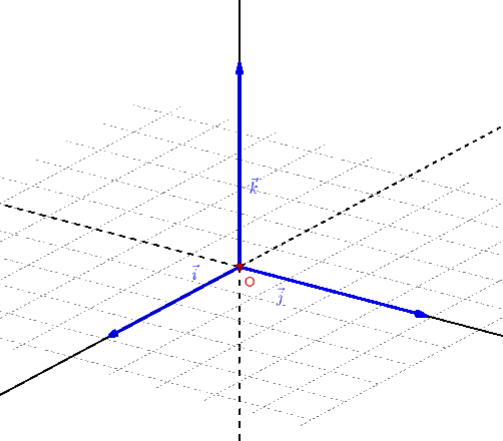
\includegraphics[width=0.7\textwidth]{./cap_estudo/dados/fig_sis_coord_orto/fig}
  \caption{Ilustração de um sistema de coordenadas ortonormal.}
  \label{fig:sis_coord_orto}
\end{figure}

Salvo explicitado diferente, trabalharemos com um \emph{sistema de coordenadas ortonormal}, i.e. sistema cuja base $B = (\vec{i},\vec{j},\vec{k})$ seja ortonormal. Mais ainda, estaremos assumindo que a base é positiva. Veja a Figura \ref{fig:sis_coord_orto}.

\subsection{Pontos e Vetores}
\badgeYouTube{NBi-Ku86pGE}

  % \href{https://archive.org/details/coordenadas-de-um-vetor}{$\blacktriangleright$ Vídeo disponível!})}
  
Seja dado um vetor $\overrightarrow{AB}$. Sabendo as coordenadas dos pontos $A = (x_A,y_A,z_A)$ e $B = (x_B,y_B,z_B)$, temos que as coordenadas do vetor $\overrightarrow{AB}$ são:
\begin{align}
  \overrightarrow{AB} &= \overrightarrow{AO} + \overrightarrow{OB}\\
                      &= -\overrightarrow{OA} + \overrightarrow{OB}\\
                      &= -(x_A,y_A,z_A)+(x_B,y_B,z_B)\\
                      &= (x_B-x_A,y_B-y_A,z_B-z_A).
\end{align}
Em uma linguagem menos formal, podemos dizer que as coordenadas de $\overrightarrow{AB}$ é a resultante das coordenadas do ponto final menos as coordenadas do ponto de partida. Veja a figura abaixo.

\begin{figure}[H]
\centering
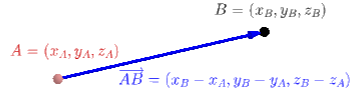
\includegraphics[width=0.6\textwidth]{./cap_estudo/dados/fig_scoord_vec_pt/fig}
\caption{Relação entre as coordenadas dos pontos de partida e de chegada de um vetor.}
\label{fig:scoord_vec_pt}
\end{figure}  

\begin{ex}
  Dados os pontos $A = (-1,1,2)$ e $B = (3,-1,0)$, temos que o vetor $\overrightarrow{AB}$ tem coordenadas:
  \begin{equation}
    \overrightarrow{AB} = (3-(-1),-1-1,0-2) = (4,-2,-2).
  \end{equation}
\end{ex}

\subsection{Ponto Médio de um Segmento}
\badgeYouTube{Yu0usAcwx5w}

% \href{https://archive.org/details/coordenadas-do-ponto-medio}{$\blacktriangleright$ Vídeo disponível!})}

Dados os pontos $A = (x_A,y_A,z_A)$ e $B = (x_B,y_B,z_B)$, podemos calcular as coordenadas do ponto médio $M = (x_M,y_M,z_M)$ do segmento $AB$. Veja a figura abaixo.

\begin{figure}[H]
\centering
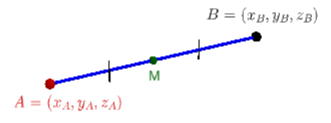
\includegraphics[width=0.6\textwidth]{./cap_estudo/dados/fig_scoord_pm/fig}
\caption{Coordenadas do ponto médio de um segmento.}
\label{fig:scoord_pm}
\end{figure}  

Do fato de que $\overrightarrow{AM} = \overrightarrow{MB}$, temos
\begin{equation}
  (x_M-x_A,y_M-y_A,z_M-z_A)=(x_B-x_M,y_B-y_M,z_B-z_M),
\end{equation}
Logo, segue que
\begin{align}
  x_M-x_A &= x_B-x_M\\
  y_M-y_A &= y_B-y_M\\
  z_M-z_A &= z_B-z_M
\end{align}
ou, equivalentemente,
\begin{align}
  2x_M &= x_A+x_B\\
  2y_M &= y_A+y_B\\
  2z_M &= z_A+z_B
\end{align}
Portanto, concluímos que
\begin{align}
  x_M &= \frac{x_A+x_B}{2}\\
  y_M &= \frac{y_A+y_B}{2}\\
  z_M &= \frac{z_A+z_B}{2}
\end{align}  
Logo, temos
\begin{equation}
M = \left(\frac{x_A+x_B}{2},\frac{y_A+y_B}{2},\frac{z_A+z_B}{2}\right)
\end{equation}

\begin{ex}
  Dados os pontos $A = (-1,1,2)$ e $B = (3,-1,0)$, temos que o ponto médio do segmento $AB$ tem coordenadas:
  \begin{align}
    M &= \left(\frac{-1+3}{2},\frac{1+(-1)}{2},\frac{2+0}{2}\right)\\
    &= (1,0,1).
  \end{align}
\end{ex}

\subsection*{Exercícios resolvidos}

\begin{exeresol}
  Sejam $A = (-1,2,1)$, $B = (1,-2,0)$ e $C = (x,2,2)$ vértices consecutivos de um triângulo isósceles, cujos lados $AC$ e $BC$ são congruentes. Determine o valor de $x$.
\end{exeresol}
\begin{resol}
  Sendo os lados $AC$ e $BC$ congruentes, temos $|\overrightarrow{AC}| = |\overrightarrow{BC}|$. As coordenadas de $\overrightarrow{AC}$ são
  \begin{equation}
    \overrightarrow{AC} = (x-(-1),2-2,2-1) = (x+1,0,1)
  \end{equation}
  e as coordenadas de $\overrightarrow{BC}$ são
  \begin{equation}
    \overrightarrow{BC} = (x-1,2-(-2),2-0) = (x-1,4,2).
  \end{equation}
  Então, temos
  \begin{align}
    |\overrightarrow{AC}| = |\overrightarrow{BC}| &\Rightarrow \sqrt{(x+1)^2+0^2+1^2} = \sqrt{(x-1)^2+4^2+2^2}\\
                                                  &\Rightarrow (x+1)^2+0^2+1^2 = (x-1)^2+4^2+2^2\\
                                                  &\Rightarrow x^2+2x+1+1 = x^2-2x+1+16+4\\
                                                  &\Rightarrow 4x = 19\\
                                                  &\Rightarrow x = \frac{19}{4}.
  \end{align}
\end{resol}

\begin{exeresol}
  Sejam $A = (-1,2,1)$, $B = (1,-2,0)$  e $M$ o ponto médio do intervalo $AB$. Determine as coordenadas do ponto $P$ de forma que $2AP = AM$.
\end{exeresol}
\begin{resol}
  As coordenadas do ponto médio são
  \begin{equation}
    M = \left(\frac{-1+1}{2},\frac{2+(-2)}{2},\frac{1+0}{2}\right) = \left(0,0,\frac{1}{2}\right).
  \end{equation}
  Agora, denotando $P = (x_P,y_P,z_P)$, temos
  \begin{align}
    2AP = AM &\Rightarrow 2(x_P-(-1),y_P-2,z_P-1) = \left(0-(-1),0-2,\frac{1}{2}-1\right)\\
             &\Rightarrow (2x_p+2,2y_P-4,2z_P-2) = \left(1,-2,-\frac{1}{2}\right).
  \end{align}
  Portanto
  \begin{align}
    & 2x_P+2 = 1 \Rightarrow x_P = -\frac{1}{2}\\
    & 2y_P-4 = -2 \Rightarrow y_P = 1\\
    & 2z_P-2 = -\frac{1}{2} \Rightarrow z_P = \frac{3}{4}.
  \end{align}
  Logo, $P = (-1/2,1,3/4)$.
\end{resol}

\subsection*{Exercícios}

\begin{exer}
  Sejam dados os pontos $A=(1,-1,2)$ e $B=(0,1,-2)$. Determine as coordenadas do vetor $\vec{v}=\overrightarrow{BA}$.
\end{exer}
\begin{resp}
  $\vec{v}=(1,-2,4)$
\end{resp}

\begin{exer}
  Sejam dados os pontos $E=(-1,2,0)$ e $F=(2,-1,1)$. Calcule o ponto médio do segmento $EF$.
\end{exer}
\begin{resp}
  $\displaystyle M=\left(\frac{1}{2},\frac{1}{2},\frac{1}{2}\right)$
\end{resp}

\begin{exer}
  Sejam dados os pontos $A=(-1,1,-1)$ e $M=(0,1,3)$. Determine o ponto $B$ tal que $M$ seja o ponto médio do segmento $AB$.
\end{exer}
\begin{resp}
  $B=(1,1,7)$
\end{resp}

\begin{exer}
  Sejam dados os pontos $A=(1,-1,1)$, $B=(2,1,0)$ e $C=(x,2,1)$. Determine $x$ tal que $ABC$ forme um triângulo retângulo com hipotenusa $BC$.
\end{exer}
\begin{resp}
  $x=-5$
\end{resp}

\begin{exer}
  Determine a distância entre os pontos $C=(2,-1,0)$ e $D=(1,1,1)$.
\end{exer}
\begin{resp}
  $|CD|=\sqrt{6}$
\end{resp}

\section{Equações da reta}\label{cap_estudo_sec_eqsreta}
\badgeRevisar

Nesta seção, vamos desenvolver equações para a representação de retas no espaço tridimensional.

\begin{figure}[H]
  \centering
  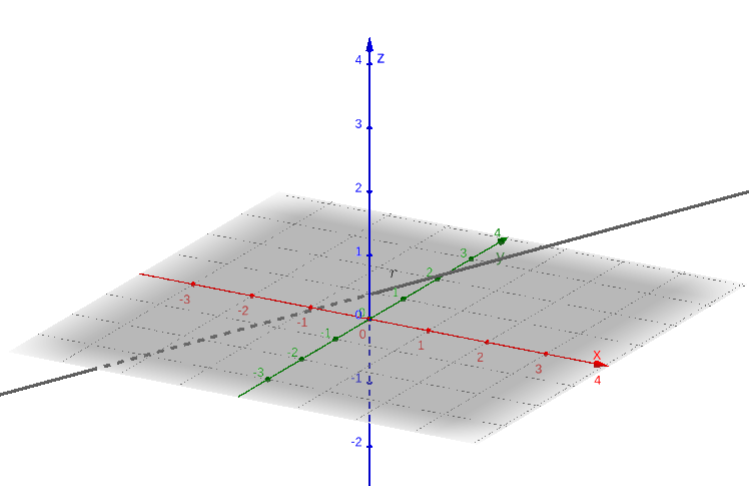
\includegraphics[width=0.8\textwidth]{cap_estudo/dados/fig_er_ilu0/fig}
  \caption{Ilustração de uma reta $r$ em um sistema de coordenadas ortonormal.}
\end{figure}

\subsection{Equação vetorial de uma reta}

Seja $r$ uma reta dada, $\vec{v}$ um vetor paralelo a $r$ e $A$ um ponto de $r$ (veja a Figura~\ref{fig:er_vet}). Assim sendo, $P=(x,y,z)$ é um ponto de $r$ se, e somente se, o vetor $\overrightarrow{AP}$ tem a mesma direção de $\vec{v}$. i.e. existe $\lambda\in\mathbb{R}$ tal que
\begin{equation}
  {\color{blue}\overrightarrow{AP} = \lambda\vec{v}}.
\end{equation}
Esta é chamada \emph{equação vetorial da reta} $r$.

\begin{figure}[H]
  \centering
  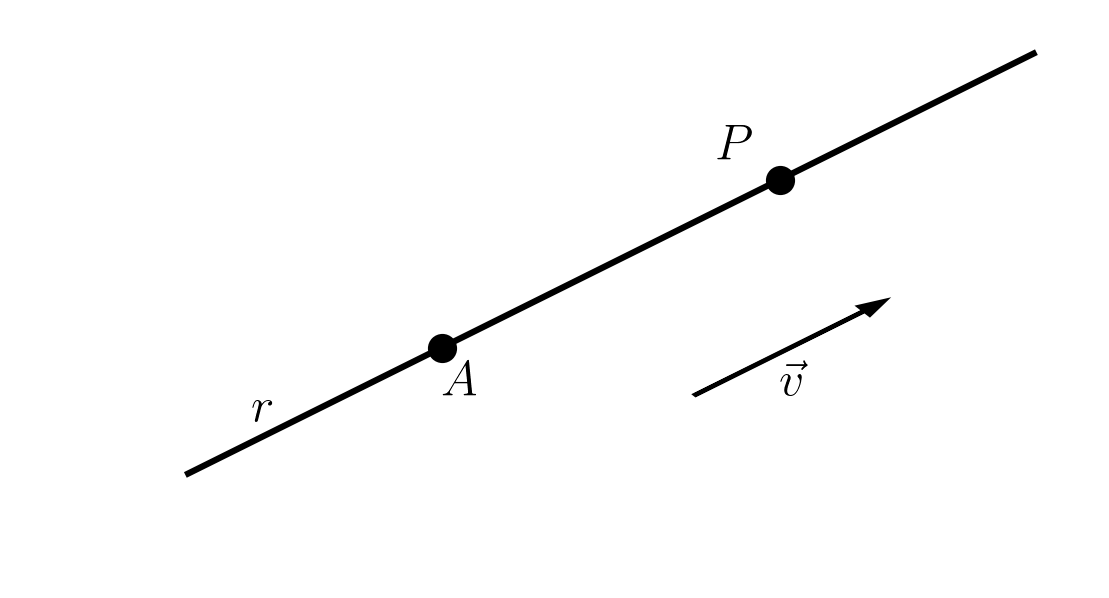
\includegraphics[width=0.5\textwidth]{./cap_estudo/dados/fig_er_vet/fig_er_vet}
  \caption{Equação vetorial de uma reta.}
  \label{fig:er_vet}
\end{figure}

Observe que para obtermos uma equação vetorial de uma dada reta, podemos escolher qualquer ponto $A\in r$ e qualquer vetor $\vec{v}\parallel r$, $\vec{v}\neq\vec{0}$. O vetor $\vec{v}$ escolhido é chamado de \emph{vetor diretor}.

\begin{ex}\label{ex:er_vet}
  Seja $r$ a reta que passa pelos pontos $A=(-1,-1,-2)$ e $B = (2,1,3)$ (veja a Figura \ref{fig:ex_er_vet}). O vetor
  \begin{equation}
    \vec{v} = \overrightarrow{AB} = (2-(-1),1-(-1),3-(-2)) = (3,2,5)
  \end{equation}
  é um vetor diretor de $r$. Desta forma, uma equação vetorial da reta $r$ é
  \begin{equation}
    \overrightarrow{AP} = \lambda\vec{v}.
  \end{equation}
  \begin{figure}[H]
    \centering
    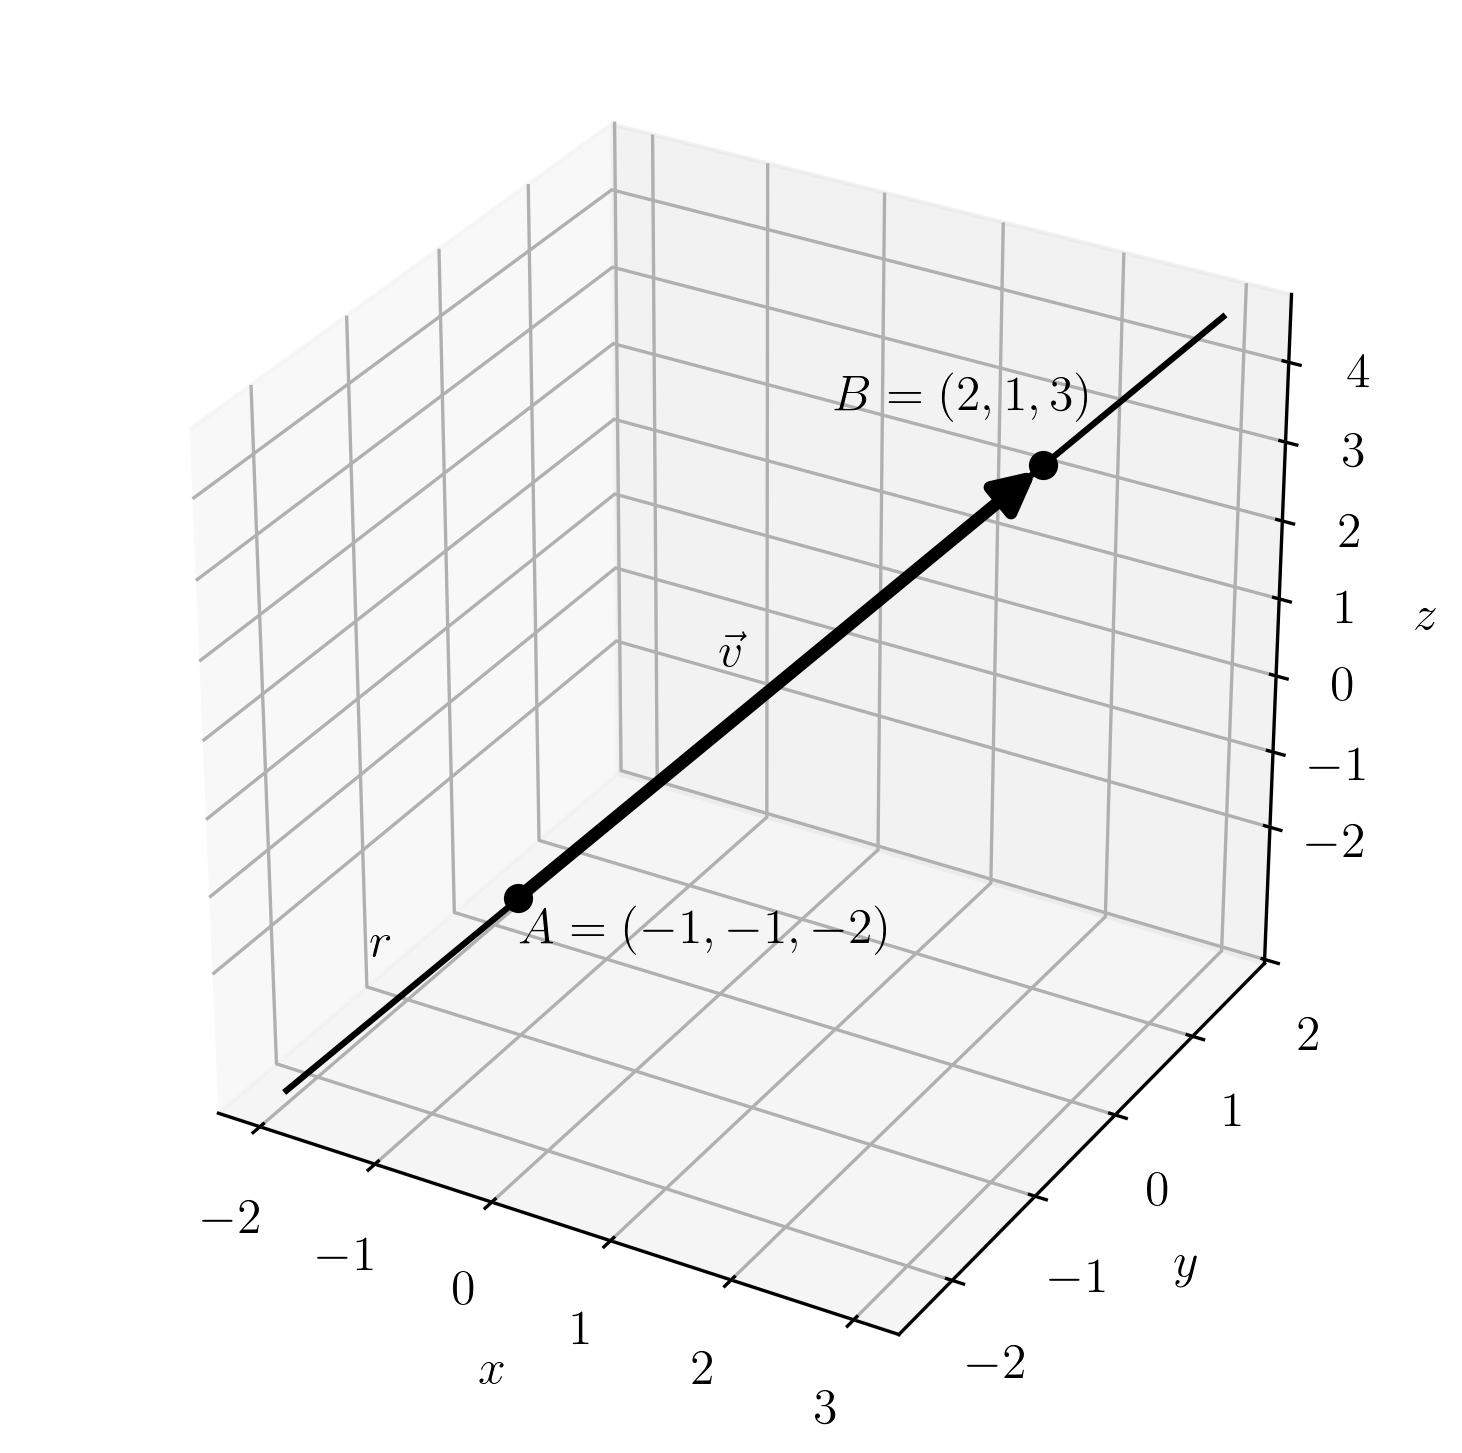
\includegraphics[width=0.7\textwidth]{./cap_estudo/dados/fig_ex_er_vet/fig_ex_er_vet}
    \caption{Esboço da reta discutida no Exemplo \ref{ex:er_vet}.}
    \label{fig:ex_er_vet}
  \end{figure}  
\end{ex}

\subsection{Equações paramétricas de uma reta}

Seja $r$ uma reta que passa pelo ponto $A = (x_A,y_A,z_A)$ e tenha vetor diretor $\vec{v} = (v_1,v_2,v_3)$. Da equação vetorial, temos que $P = (x,y,z)\in r$ se, e somente se, existe $\lambda\in\mathbb{R}$ tal que
\begin{equation}
  \overrightarrow{AP} = \lambda\vec{v}.
\end{equation}
Equivalentemente,
\begin{equation}
  \underbrace{(x-x_A,y-y_A,z-z_A)}_{\overrightarrow{AP}} = \lambda \underbrace{(v_1,v_2,v_3)}_{\vec{v}}.
\end{equation}
Então,
\begin{align}
  x-x_A &= \lambda v_1,\\
  y-y_A &= \lambda v_2,\\
  z-z_A &= \lambda v_3,
\end{align}
donde
\begin{align}
  {\color{blue}x} &{\color{blue}= x_A + \lambda v_1},\\
  {\color{blue}y} &{\color{blue}= y_A + \lambda v_2},\\
  {\color{blue}z} &{\color{blue}= z_A + \lambda v_3},
\end{align}
as quais são chamadas de \emph{equações paramétricas} da reta $r$.

\begin{ex}\label{ex:ex_er_par}
  A reta $r$ discutida no Exemplo \ref{ex:er_vet} tem equações paramétricas
  \begin{align}
    x &= -1 + 3\lambda,\\
    y &= -1 + 2\lambda,\\
    z &= -2 + 5\lambda.
  \end{align}
  De fato, tomando $\lambda = 0$, temos $(x,y,z) = (-1,-1,-2) = A\in r$. E, tomado $\lambda = 1$, temos $(x,y,z) = (-1+3,-1+2,-2+5) = (2,1,3) = B\in r$. Ou seja, as equações paramétricas acima representam a reta que passa pelos pontos $A$ e $B$.

  \ifispython
  Com o \verb+Sympy+, podemos plotar o gráfico de $r$ usando o seguinte código:
\begin{verbatim}
var('lbda',real=True)
plot3d_parametric_line(-1+3*lbda,-1+2*lbda,-2+5*lbda,(lbda,-1,2))
\end{verbatim}
  \fi
\end{ex}

\subsection{Equações da reta na forma simétrica}

Seja $r$ uma reta que passa pelo ponto $A = (x_A,y_A,z_A)$ e tem $\vec{v} = (v_1,v_2,v_3)$ como vetor diretor. Então, $r$ tem as equações paramétricas
\begin{align}
  x &= x_A + v_1\lambda,\\
  y &= y_A + v_2\lambda,\\
  z &= z_A + v_3\lambda.
\end{align}
Isolando $\lambda$ em cada uma das equações, obtemos
\begin{align}
  \lambda &= \frac{x-x_A}{v_1},\\
  \lambda &= \frac{y-y_A}{v_2},\\
  \lambda &= \frac{z-z_A}{v_3}.
\end{align}
Daí, temos
\begin{equation}
  {\color{blue}\frac{x-x_A}{v_1} = \frac{y-y_A}{v_2} = \frac{z-z_A}{v_3}},
\end{equation}
as quais são as \emph{equações da reta na forma simétrica}.

\begin{ex}
  No Exemplo \ref{ex:ex_er_par}, consideramos a reta $r$ de equações paramétricas
  \begin{align}
    x &= -1 + 3\lambda,\\
    y &= -1 + 2\lambda,\\
    z &= -2 + 5\lambda.    
  \end{align}
  Para obtermos as equações de $r$ na forma simétrica, basta isolarmos $\lambda$ em cada equação. Com isso, obtemos
  \begin{equation}
    \frac{x+1}{3} = \frac{y+1}{2} = \frac{z+2}{5}.
  \end{equation}
\end{ex}

\subsection*{Exercícios resolvidos}

\begin{exeresol}
  Seja $r$ a reta que passa pelo ponto $A = (-1,-1,-2)$ e tem $\vec{v} = (3,2,5)$ como vetor diretor. Determine o valor de $x$ de forma que $P = \left(x, 0, \frac{1}{2}\right)$ seja um ponto de $r$.
\end{exeresol}
\begin{resol}
  Da equação vetorial da reta $r$, temos que $P = \left(x,0,\frac{1}{2}\right)$ é um ponto de $r$ se, e somente se, existe $\lambda\in\mathbb{R}$ tal que
  \begin{equation}
    \overrightarrow{AP} = \lambda\vec{v}.
  \end{equation}
  Ou seja,
  \begin{equation}
    \left(x-(-1),0-(-1),\frac{1}{2}-(-2)\right) = \lambda (3,2,5).
  \end{equation}
  Ou, equivalentemente,
  \begin{equation}
    \left(x+1,1,\frac{5}{2}\right) = \lambda (3,2,5).
  \end{equation}
  Usando a segunda coordenada destes vetores, temos
  \begin{gather}
    1 = \lambda\cdot 2\\
    \lambda = \frac{1}{2}.
  \end{gather}
  Assim, da primeira coordenada dos vetores, temos
  \begin{gather}
    x+1 = \lambda\cdot 3 \\
    x+1 = \frac{1}{2}\cdot 3\\
    x = \frac{3}{2}-1\\
    x= \frac{1}{2}.
  \end{gather}
\end{resol}

\begin{exeresol}
  Seja $r$ a reta de equações paramétricas
  \begin{align}
    x &= 1 -\lambda,\\
    y &= \lambda,\\
    z &= -3.
  \end{align}
  Determine uma equação vetorial de $r$.
\end{exeresol}
\begin{resol}
  Nas equações paramétricas de uma reta, temos que os coeficientes constantes estão associados a um ponto da reta. Os coeficientes do parâmetro $\lambda$ estão associados a um vetor diretor. Assim sendo, das equações paramétricas da reta $r$, temos que
  \begin{equation}
    A = (1,0,-3)\in r
  \end{equation}
  e
  \begin{equation}
    \vec{v} = (-1,1,0)
  \end{equation}
  é um vetor diretor. Logo, temos que a reta $r$ tem equação vetorial
  \begin{equation}
    \overrightarrow{AP} = \lambda\vec{v},
  \end{equation}
  com $A = (1,0,3)$ e $\vec{v} = (-1,1,0)$.
\end{resol}

\begin{exeresol}
  Sabendo que $r$ é uma reta que passa pelos pontos $A = (2,-3,1)$ e $B = (-1,1,0)$, determine o valor de $t$ tal que
  \begin{align}
    x &= 2 + t\lambda,\\
    y &= -2 + 4\lambda,\\
    z &= 1 -\lambda,
  \end{align}
  sejam equações paramétricas de $r$.
\end{exeresol}
\begin{resol}
  Para que estas sejam equações paramétricas de $r$, é necessário que $\vec{v} = (t,4,-1)$ seja um vetor diretor de $r$. Em particular, $\vec{v} \parallel \overrightarrow{AB}$. Logo, existe $\beta\in\mathbb{R}$ tal que
  \begin{gather}
    \vec{v} = \beta\overrightarrow{AB}\\
    (t,4,-1) = \beta (-1-2,1-(-3),0-1) \\
    (t,4,-1) = \beta (-3,4,-1).
  \end{gather}
  Das segunda e terceira coordenadas, temos $\beta = 1$. Daí, comparando pela primeira coordenada, temos
  \begin{gather}
    t = -3\beta\\
    t = -3.
  \end{gather}
\end{resol}

\begin{exeresol}\label{exeresol:er_sim}
  Seja $r$ uma reta de equações na forma simétrica
  \begin{equation}
    \frac{x+1}{2} = \frac{y-2}{3} = \frac{1-z}{2}.
  \end{equation}
  Determine equações paramétricas para esta reta e faça um esboço de seu gráfico.
\end{exeresol}
\begin{resol}
  Podemos obter equações paramétricas desta reta a partir de suas equações na forma simétrica. Para tanto, basta tomar o parâmetro $\lambda$ tal que
  \begin{align}
    \lambda &= \frac{x+1}{2},\\
    \lambda &= \frac{y-2}{3},\\
    \lambda &= \frac{1-z}{2}.
  \end{align}
  Daí, isolando $x$, $y$ e $z$ em cada uma destas equações, obtemos
  \begin{align}
    x &= -1 + 2\lambda,\\
    y &= 2 + 3\lambda,\\
    z &= 1 - 2\lambda.
  \end{align}
  Para fazermos um esboço do gráfico desta reta, basta traçarmos a reta que passa por dois de seus pontos. Por exemplo, tomando $\lambda = 0$, temos $A = (-1,2,1)\in r$. Agora, tomando $\lambda = 1$, temos $B = (1,5,-1)\in r$. Desta forma, obtemos o esboço dado na Figura \ref{fig:exeresol_er_sim}.

  \begin{figure}[H]
    \centering
    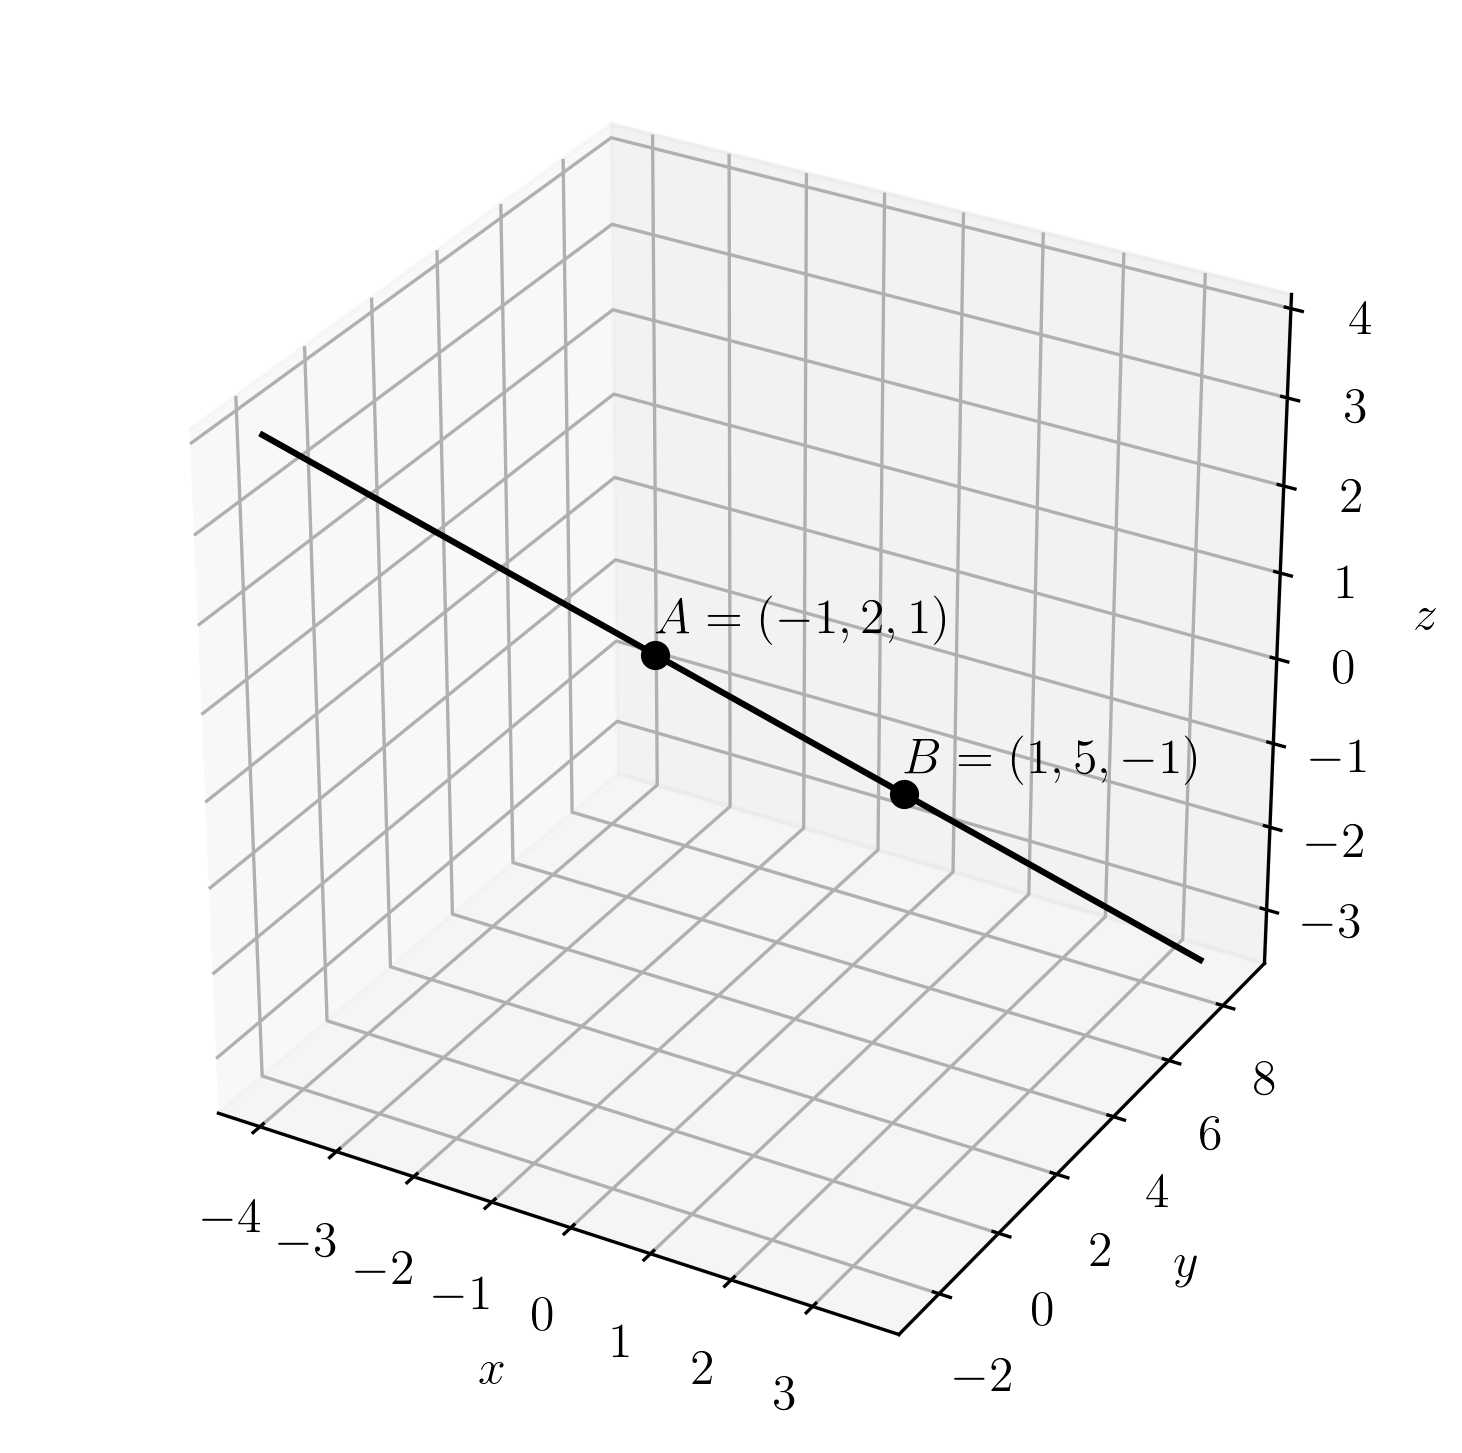
\includegraphics[width=0.7\textwidth]{./cap_estudo/dados/fig_exeresol_er_sim/fig_exeresol_er_sim}
    \caption{Esboço do gráfico da reta $r$ do Exercício Resolvido \ref{exeresol:er_sim}.}
    \label{fig:exeresol_er_sim}
  \end{figure}
\end{resol}

\subsection*{Exercícios}

\begin{exer}
  Seja a reta que passa pelos pontos $A=(1,-2,0)$ e $B=(-1,-1,1)$. Determine:
  \begin{enumerate}[a)]
  \item sua equação vetorial.
  \item suas equações paramétricas.
  \item suas equações na forma simétrica.
  \end{enumerate}
\end{exer}
\begin{resp}
  a) $\overrightarrow{AP}=\lambda\vec{v}$, $\vec{v}=(-2,1,1)$; b) $x=1-2\lambda$, $y=-2+\lambda$, $z=\lambda$; c) $\frac{x-1}{-2}=y+2=z$
\end{resp}

\begin{exer}
  Seja a reta que passa pelo ponto $A=(0,1,-1)$ e tem vetor diretor $\vec{v}=(2,-1,1)$. Determine $x$ tal que $B=(1,x,-\frac{1}{2})$.
\end{exer}
\begin{resp}
  $x=\frac{1}{2}$
\end{resp}

\begin{exer}
  Considere a reta de equações na forma simétrica
  \begin{equation}
    \frac{x-1}{-2}=\frac{y+1}{3}=z-1.
  \end{equation}
  Encontre um ponto e um vetor diretor desta reta.
\end{exer}
\begin{resp}
  $A=(1,-1,1)$, $\vec{v}=(-2,3,1)$
\end{resp}

\begin{exer}
  Seja a reta $r$ de equações paramétricas
  \begin{align}
    x &= \lambda\\
    y &= 2-\lambda\\
    z &= -1+\lambda
  \end{align}
  Determine as equações na forma simétrica da reta que passa pelo ponto $A=(1,-1,0)$ e é paralela a reta $r$.
\end{exer}
\begin{resp}
  $x-1=\frac{y+1}{-1}=z$
\end{resp}

\begin{exer}
  Seja a reta $r$ de equações paramétricas
  \begin{align}
    x &= \lambda\\
    y &= 2-\lambda\\
    z &= -1+\lambda
  \end{align}
  Determine as equações paramétricas da reta que passa pelo ponto $A=(1,-1,0)$ e é perpendicular a reta $r$.
\end{exer}
\begin{resp}
  $x=1-\lambda$, $y=-1-2\lambda$, $z=-\lambda$
\end{resp}

\section{Equações do plano}\label{cap_estudo_sec_eqsplano}
\badgeRevisar

Um plano $\pi$ fica unicamente determinado por um ponto $A\in \pi$ e dois vetores linearmente independentes $\vec{u},\vec{v}\in \pi$\footnote{No sentido que $\vec{u}$ e $\vec{v}$ têm representantes no plano $\pi$.}. Veja a Figura \ref{fig:ep_plano}.

\begin{figure}[H]
  \centering
  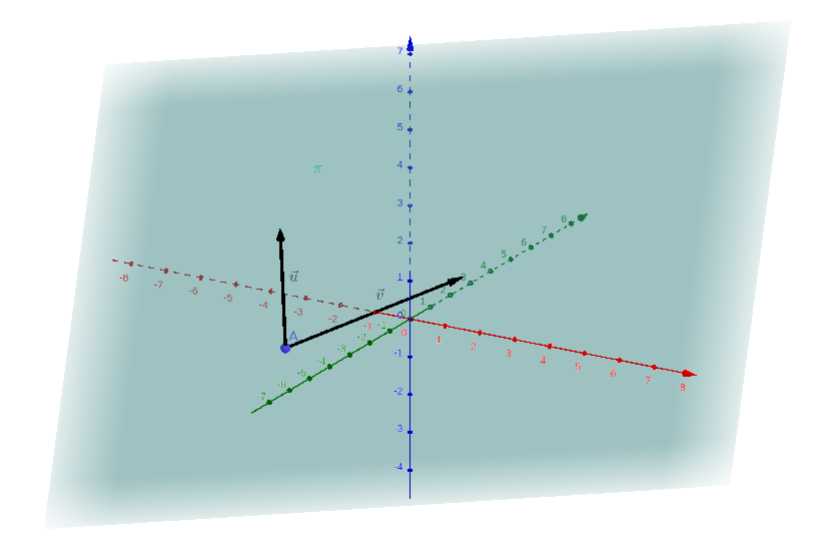
\includegraphics[width=0.9\textwidth]{cap_estudo/dados/fig_ep_plano/fig}
  \caption{Ilustração de um plano no espaço tridimensional.}
  \label{fig:ep_plano}
\end{figure}

Os chamados \emph{vetores diretores} $\vec{u}$ e $\vec{v}$ determinam infinitos planos paralelos entre si. O chamado \emph{ponto de ancoragem} $A$ fixa um destes planos.

\subsection{Equação vetorial do plano}

Consideremos um plano $\pi$ determinado pelo ponto de ancoragem $A$ e os vetores diretores $\vec{u}$ e $\vec{v}$ (veja a Figura \ref{fig:ep_evp}). Então, um ponto $P\in \pi$ se, e somente se, $\overrightarrow{AP}$ é coplanar a $\vec{u}$ e $\vec{v}$, i.e. $\overrightarrow{AP}$, $\vec{u}$ e $\vec{v}$ são linearmente dependentes. Ou seja, $P\in\pi$ se, e somente se, $\overrightarrow{AP}$ pode ser escrito como combinação linear de $\vec{u}$ e $\vec{v}$. Isto nos fornece a chamada \emph{equação vetorial do plano}
\begin{equation}
  {\color{blue}P\in\pi \Leftrightarrow \overrightarrow{AP} = \lambda\vec{u}+\beta\vec{v},\quad\lambda,\beta\in\mathbb{R}}.
\end{equation}

\begin{figure}[H]
  \centering
  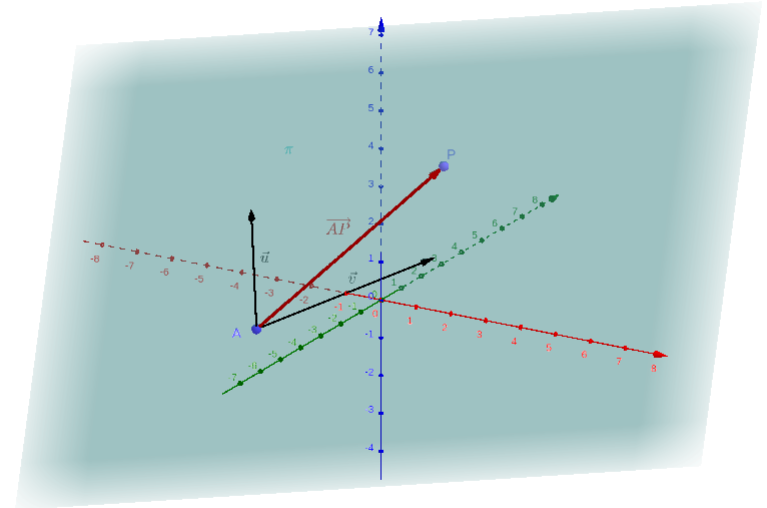
\includegraphics[width=0.9\textwidth]{cap_estudo/dados/fig_ep_evp/fig}
  \caption{Ilustração sobre a equação vetorial de um plano.}
  \label{fig:ep_evp}
\end{figure}


\begin{ex}\label{ex:ep_vet}
  Consideremos o plano $\pi$ determinado pelo ponto $A = (1,-1,1)$ e pelos vetores $\vec{u} = (2,-1,0)$ e $\vec{v} = (0,1,1)$ (Veja a Figura \ref{fig:ex_ep_vet}. Desta forma, uma equação vetorial para este plano é
  \begin{equation}
    \overrightarrow{AP} = \lambda\vec{u}+\beta\vec{v},
  \end{equation}
  para $\lambda,\beta\in\mathbb{R}$.
  
  \begin{figure}[H]
    \centering
    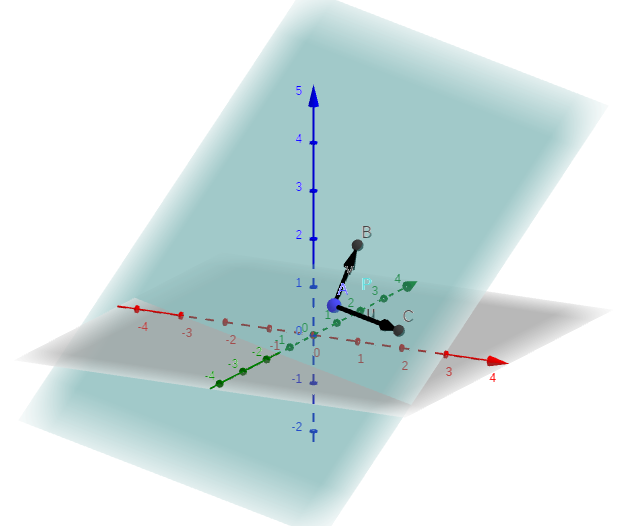
\includegraphics[width=0.9\textwidth]{./cap_estudo/dados/fig_ex_ep_vet/fig_ex_ep_vet}
    \caption{Esboço do plano $\pi$ discutido no Exemplo \ref{ex:ep_vet}.}
    \label{fig:ex_ep_vet}
  \end{figure}
  
  Tomando, por exemplo, $\lambda = -1$ e $\beta = 1$, obtemos
  \begin{align}
    \overrightarrow{AP} &= \lambda\vec{u}+\beta\vec{v}\\
                        &= -(2,-1,0) + (0,1,1)\\
                        &= (-2,2,1).
  \end{align}
  Observando que as coordenadas do ponto $P$ são iguais as coordenadas do vetor $\overrightarrow{OP}$, temos
  \begin{align}
    \overrightarrow{OP} &= \overrightarrow{OA}+\overrightarrow{AP}\\
                        &= (1,-1,1)+(-2,2,1)\\
                        &= (-1,1,2).
  \end{align}
  Ou seja, $P = (-1,1,2)\in\pi$.
\end{ex}

\subsection{Equações paramétricas do plano}

Seja um plano $\pi$ com ponto de ancoragem $A=(x_A,y_A,z_A)\in\pi$ e vetores diretores $\vec{u}=(u_1,u_2,u_3)$ e $\vec{v}=(v_1,v_2,v_3)$. Então, todo o ponto $P=(x,y,z)$ neste plano $\pi$ satisfaz a equação vetorial
\begin{equation}
  \overrightarrow{AP} = \lambda\vec{u}+\beta\vec{v},
\end{equation}
para dados parâmetros $\lambda,\beta\in\mathbb{R}$. Assim, temos
\begin{align}
  (x-x_A,y-y_A,z-z_A) &= \lambda(u_1,u_2,u_3)+\beta(v_1,v_2,v_3)\\
                      &= (\lambda u_1+\beta v_1,\lambda u_2+\beta v_2,\lambda u_3+\beta v_3).
\end{align}
Portanto, temos
\begin{align}
  x-x_A &= \lambda u_1+\beta v_1,\\
  y-y_A &= \lambda u_2+\beta v_2,\\
  z-z_A &= \lambda u_3+\beta v_3.
\end{align}
Ou, equivalentemente,
\begin{align}
  {\color{blue}x} &= {\color{blue}x_A + \lambda u_1+\beta v_1},\\
  {\color{blue}y} &= {\color{blue}y_A + \lambda u_2+\beta v_2},\\
  {\color{blue}z} &= {\color{blue}z_A + \lambda u_3+\beta v_3},
\end{align}
as quais são chamadas de \emph{equações paramétricas do plano}.

\begin{ex}
  No Exemplo \ref{ex:ep_vet}, discutimos sobre o plano $\pi$ determinado pelo ponto $A = (1,-1,1)$ e os vetores $\vec{u}=(2,-1,0)$ e $\vec{v}=(0,1,1)$. Do que vimos acima, temos que
  \begin{align}
    x &= 1 + 2\lambda,\\
    y &= -1 -\lambda + \beta,\\
    z &= 1+\beta,
  \end{align}
  são equações paramétricas deste plano.

  \ifispython
  Podemos usar as equações paramétricas do plano para plotá-lo usando o \sympy. Para tanto, podemos usar os seguintes comandos:
\begin{verbatim}
from sympy import *
from sympy.plotting import plot3d_parametric_surface
var('r,s',real=True)
plot3d_parametric_surface(1+2*r,-1-r+s,1+s,
                          (r,-2,2),(s,-2,2),show=True,
                          xlabel='$x$',ylabel='$y$')
\end{verbatim}
  \fi
\end{ex}

\subsection{Equação geral do plano}

Seja $\pi$ o plano determinado pelo ponto de ancoragem $A=(x_A,y_A,z_A)$ e pelos vetores diretores $\vec{u}=(u_1,u_2,u_3)$ e $\vec{v} = (v_1,v_2,v_3)$. Sabemos que $P=(x,y,z)\in\pi$ se, e somente se, $\overrightarrow{AP}$, $\vec{u}$ e $\vec{v}$ são linearmente dependentes. Ou, equivalentemente, o produto misto $[\overrightarrow{AP},\vec{u},\vec{v}] = 0$. Logo,
\begin{align}
  0 &= [\overrightarrow{AP},\vec{u},\vec{v}] \\
    &=
      \begin{vmatrix}
        x-x_A & y-y_A & z-z_A \\
        u_1 & u_2 & u_3 \\
        v_1 & v_2 & v_3
      \end{vmatrix} \\
    &= -u_1v_2z_A + u_1v_3y_A + u_2v_1z_A \\
    &- u_2v_3x_A - u_3v_1y_A + u_3v_2x_A \\
    &+ x{\color{blue}(u_2v_3 - u_3v_2)} + y{\color{red}(-u_1v_3 + u_3v_1)} + z{\color{orange}(u_1v_2 - u_2v_1)}.
\end{align}
Observamos que a equação acima tem a forma geral
\begin{equation}
  {\color{blue}a}x + {\color{red}b}y + {\color{orange}c}z + d = 0,
\end{equation}
com $a,b,c,d$ não todos nulos ou, equivalentemente, $a^2+b^2+c^2+d^2\neq 0$. Esta última é chamada \emph{equação geral do plano}.

\begin{ex}
  No Exemplo \ref{ex:ep_vet}, discutimos sobre o plano $\pi$ determinado pelo ponto $A = (1,-1,1)$ e os vetores $\vec{u}=(2,-1,0)$ e $\vec{v}=(0,1,1)$. Para encontrarmos a equação geral deste plano, tomamos $P = (x,y,z)$ e calculamos
  \begin{align}
    0 &= [\overrightarrow{AP},\vec{u},\vec{v}]\\
      &=
        \begin{vmatrix}
          x-1 & y+1 & z-1 \\
          2 & -1 & 0 \\
          0 & 1 & 1
        \end{vmatrix}\\
      &= - x - 2 y + 2 z - 3.
  \end{align}
  Ou seja, a equação geral deste plano é
  \begin{equation}
    -x - 2y + 2z -3 = 0.
  \end{equation}
\end{ex}

\subsection{Exercícios resolvidos}

\begin{exeresol}
  Seja $\pi$ um plano tal que $A=(2,0,-1)\in\pi$, $P=(0,1,-1)\in\pi$ e $\vec{u}=(1,0,1)\in\pi$. Determine uma equação vetorial para $\pi$.
\end{exeresol}
\begin{resol}
  Para obtermos uma equação vetorial do plano $\pi$, precisamos de um ponto e dois vetores l.i. em $\pi$. Do enunciado, temos o ponto $A=(2,0,-1)\in\pi$ e o vetor $\vec{u}$. Portanto, precisamos encontrar um vetor $\vec{v}\in\pi$ tal que $\vec{u}$ e $\vec{v}$ sejam l.i.. Por sorte, temos $P=(0,1,-1)\in\pi$ e, portanto $\overrightarrow{AP}\in\pi$. Podemos tomar
  \begin{align}
    \vec{v} &= \overrightarrow{AP}\\
            &= (-2,1,0),
  \end{align}
  pois $\vec{v}$ e $\vec{u}$ são l.i.. Logo, uma equação vetorial do plano $\pi$ é
  \begin{align}
    \overrightarrow{AP} &= \lambda\vec{u}+\beta\vec{v},\\
                        &= \lambda (1,0,1) + \beta (-2,1,0),
  \end{align}
  com $\lambda,\beta\in\mathbb{R}$.
\end{resol}

\begin{exeresol}
  Seja $\pi$ o plano de equações paramétricas
  \begin{align}
    x = -1 + \lambda,\\
    y = \beta,\\
    z = 1 - \lambda + \beta.
  \end{align}
  Determine o valor de $z_P$ de forma que $P=(-1,2,z_P)\in\pi$.
\end{exeresol}
\begin{resol}
  Para que $P=(-1,2,z_P)$ pertença ao plano, devemos ter
  \begin{align}
    -1 = -1 + \lambda,\\
    2 = \beta,\\
    z_P = 1 - \lambda + \beta.
  \end{align}
  Das duas primeiras equações, obtemos $\lambda=0$ e $\beta=2$. Daí, da terceira equação, temos
  \begin{align}
    z_P = 1 - 0 + 2 = 3.
  \end{align}
\end{resol}

\subsection*{Exercícios}

\begin{exer}
  Determine a equação vetorial do plano com ponto de ancoragem $A=(-1,0,2)$ e vetores diretores $\vec{u}=(2,-1,1)$ e $\vec{v}=(-1,1,2)$.
\end{exer}
\begin{resp}
  $\overrightarrow{AP}=\lambda(2,-1,1)+\beta(-1,1,2),\quad\lambda,\beta\in\mathbb{R}$
\end{resp}

\begin{exer}
  Seja o plano de equação vetorial $\overrightarrow{AP}=\lambda(2,-1,1)+\beta(-1,1,2)$, $\lambda,\beta\in\mathbb{R}$, com ponto de ancoragem $A=(-1,0,2)$. Determine $x$ tal que $P=(x,3,0)$ pertença a este plano.
\end{exer}
\begin{resp}
  $x=5$
\end{resp}

\begin{exer}
  Determine as equações paramétricas do plano com ponto de ancoragem $A=(-1,0,2)$ e vetores diretores $\vec{u}=(2,-1,1)$ e $\vec{v}=(-1,1,2)$.
\end{exer}
\begin{resp}
  $x=-1+2\lambda - \beta$, $y=-\lambda+\beta$, $z=2+\lambda+2\beta$
\end{resp}

\begin{exer}
  Considere o plano de equações paramétricas
  \begin{align}
    x &= -1+2\lambda - \beta,\\
    y &= -\lambda+\beta,\\
    z &= 2+\lambda+2\beta.
  \end{align}
  Determine $y$ tal que $P=(-6,y,2)$ pertença a este plano.
\end{exer}
\begin{resp}
  $y=3$
\end{resp}

\begin{exer}
  Determine a equação geral do plano com ponto de ancoragem $A=(-1,0,2)$ e vetores diretores $\vec{u}=(2,-1,1)$ e $\vec{v}=(-1,1,2)$.
\end{exer}
\begin{resp}
  $-3x -5y + z - 5 = 0$
\end{resp}

\begin{exer}
  Considere o plano de equação geral $-3x -5y + z - 5 = 0$. Determine $z$ tal que o ponto $P=(0,0,z)$ pertença a este plano.
\end{exer}
\begin{resp}
  $z=5$
\end{resp}

\begin{exer}
  Considere o plano $\pi$ de equações paramétricas
  \begin{align}
    x &= -1 + \lambda\\
    y &= \beta \\
    z = &= 1 - \lambda + \beta
  \end{align}
  A reta $r$ de equação paramétricas
  \begin{align}
    x &= 2\\
    y &= -1 + 2\lambda\\
    z &= 2\lambda
  \end{align}
  é paralela ao plano $\pi$? Justifique sua resposta.
\end{exer}
\begin{resp}
  sim
\end{resp}

\begin{exer}
  Considere o plano $\pi$ de equação geral
  \begin{equation}
    6x -7y - 5z = -6.
  \end{equation}
  Determine uma equação paramétrica para a reta $r$ que é perpendicular ao plano $\pi$ e passa pelo ponto $A=(2,-1,0)$.
\end{exer}
\begin{resp}
  $x=2+6\lambda$, $y=-1-7\lambda$, $z=-5\lambda$
\end{resp}
